
\subsection{Background}
    The first paradigm used to solve the VLSI optimization problem is Constraint Programming (CP),
    developed using MiniZinc as modeling language. 
    Starting from a base model following the constraints discussed in \ref{sec:shared_constraints},
    we added: rotation variables $r_i$, symmetry breaking constraints and search strategies;
    to be more precise we have a model for each combination of the previous elements.
    To test different behaviour of solvers we have chosen to run each model on both Chuffed and Gecode solvers.

% % % % % % % % % % % % % % % % % % % % % % % % % % % % % % % % % % % % % % % % % % % % % % % % % %

\subsection{Notation} \label{sec:CP_notation}
    In CP we tried to break also the symmetries related to \textit{virtual} circuits, but, as already
    explained in section \ref{sec:symmetries}, we decided to keep only the simplest ones that will 
    be described soon.

    This section is mainly needed to introduce constans related to \textit{virtual} circuits:
    
    \begin{align*}
        vc_{i,j}    &\ =\ \text{\textit{virtual} circuit obtained from  } (i,j) \in CC      \\
        n\_vc\      &\ =\ \text{maximum number of \textit{virtual} circuits}                \\
                    &\ =\ |CC| = \frac{nc!}{2! \cdot (nc - 2)!} = \frac{nc \cdot (nc-1)}{2} \\
        n\_rvc\     &\ =\ n\_vc + nc                                                        \\
        VC          &\ =\ \{ c_i\ |\ i \in [1,n\_vc] \}                                     \\
        VV          &\ =\ \{ (i,j)\ \in VC \times VC |\ i <j \}                             \\
        RVC         &\ =\ \{ c_i\ |\ i \in [1,n\_rvc] \}                                    \\
        % c_pairs &\ =\ [(i,j)\ |\ (i,j) \in CC]
    \end{align*}

    The first definition needs deeper explanation: a rectangle can be defined giving the position
    of its bottom left and its top right corner and for a \textit{virtual} circuit they are the
    bottom left corner of circuit $i$ and the top right corner of circuit $j$.
    The maximum number of virtual circuit is then given by the combinations (without repetition)
    of two circuit indexes, which is also the cardinality of $CC$. 

    

% % % % % % % % % % % % % % % % % % % % % % % % % % % % % % % % % % % % % % % % % % % % % % % % % %

\subsection{Functions \& Predicates}
    The additional functions and predicates we define in this section will later be used in the models
    adopting symmetry breaking constraints and the ones allowing rotation of circuits; the others work 
    with the constraints already defined in \ref{sec:shared_constraints}.
    
    \paragraph{Functions}
    \begin{align}
        vc\_x(vc_{i,j})\        =\ & min(x_i, x_j)                                                  \\
        vc\_y(vc_{i,j})\        =\ & min(y_i, y_j)                                                  \\
        vc\_width(vc_{i,j})\    =\ & max(x_i + w_i, x_j + w_j) - vc\_x(vc_{i,j})                    \\
        vc\_height(vc_{i,j})\   =\ & max(y_i + h_i, y_j + h_j) - vc\_y(vc_{i,j})                    \\
        r\_w(c) =\  & bool2int(\neg\ is\_rotated_c) \cdot w_c + bool2int(is\_rotated_c) \cdot h_c   
        \label{eq:CP_r_w}   \\
        r\_h(c) =\  & bool2int(\neg\ is\_rotated_c) \cdot h_c + bool2int(is\_rotated_c) \cdot w_c   
        \label{eq:CP_r_h}
    \end{align}

    where $vc\_x(vc_{i,j})$, $vc\_y(vc_{i,j})$, $vc\_width(vc_{i,j})$ and $vc\_height(vc_{i,j})$ 
    return respectively the $x$, $y$, $w$ and $h$ of the \textit{virtual} circuit $vc_{i,j}$, while 
    $r\_w(c)$ and $r\_h(c)$ check if circuit $c$ is rotated and update coherently $w_c$ and $h_c$.

    \paragraph{Predicates}
    \begin{align*}
        vc\_is\_valid(vc_{i,j})     &\leftarrow\    \bigwedge_{c \in C} &  (\neg(x_c < vc_x \land x_c + w_c > vc_x) \land
                                                    \neg(x_c + w_c > vc_x + vc_w))                                  \\
                                                &&  \lor                                             \\
                                                &&  (\neg(y_c < vc_y \land y_c + h_c > vc_y) \land
                                                    \neg(y_c + h_c > vc_y + vc_h))                                  \\
        c\_equal\_dim\_symmetry &\leftarrow\        \bigwedge_{(c_1, c_2) \in CC} & (w_{c_1} == w_{c_2} \land h_{c_1} == h_{c_2})                   \\
                                                &&  \rightarrow lex\_lesseq([x_{c_1}, y_{c_1}], [x_{c_2}, y_{c_2}]) \\ 
        vc\_equal\_dim\_symmetry &\leftarrow\       \bigwedge_{(c, vc) \in C \times VC} & (vc\_is\_valid(vc) \land w_{c_1} == w_{c_2} \land h_{c_1} == h_{c_2})   \\
                                                &&  \rightarrow lex\_lesseq([x_{c_1}, y_{c_1}], [x_{c_2}, y_{c_2}])     \\      
        vv\_equal\_dim\_symmetry &\leftarrow\       \bigwedge_{(vc_1, vc_2) \in VV}
                                                &   (vc\_is\_valid(vc_1) \land vc\_is\_valid(vc_2) \land                         \\
                                                &&  \neg (vc_{1x} == vc_{2x}) \land \\
                                                &&  vc_{1w} == vc_{2w} \land vc_{1h} == vc_{2h} \land \\
                                                &&  (|vc_{1x} - vc_{2x}| \geq vc_{1w} lor |vc_{1y} - vc_{2y}| \geq vc_{1h})) \\
                                                &&  \rightarrow lex\_lesseq([vc_{1x}, vc_{1y}], [vc_{2x}, vc_{2y}]) \\
        c\_consecutive\_on\_x(c_1, c_2) &\leftarrow  &   x_{c_1} + w_{c_1} == x_{c_2} \lor x_{c_2} + w_{c_2} == x_{c_1} \\
        c\_consecutive\_on\_y(c_1, c_2) &\leftarrow  &   y_{c_1} + h_{c_1} == y_{c_2} \lor y_{c_2} + h_{c_2} == y_{c_1} \\
        c\_can\_be\_swapped\_on\_x(c_1, c_2) &\leftarrow & c\_consecutive\_on\_x(c_1, c_2) \land y_{c_1} == y_{c_2} \land h_{c_1} == h_{c_2} \\
        c\_can\_be\_swapped\_on\_y(c_1, c_2) &\leftarrow & c\_consecutive\_on\_y(c_1, c_2) \land x_{c_1} == x_{c_2} \land w_{c_1} == w_{c_2} \\ 
        c\_consecutive\_symmetry &\leftarrow  \bigwedge_{(c_1, c_2) \in CC} & (c\_can\_be\_swapped\_on\_x(c_1, c_2) \rightarrow lex\_less([ x_{c_1} ], [ x_{c_2} ])) \land \\
                                                &&  (c\_can\_be\_swapped\_on\_y(c_1, c_2) \rightarrow lex\_less([ y_{c_1} ], [ y_{c_2} ]))     
    \end{align*}
    As mentioned in \ref{sec:CP_notation}, $vc_{i,j}$ defines a rectangle in the plate, but, in order to 
    be defined as \textit{virtual} circuit, its edges must not cross any regular circuit. 
    This condition is checked by the predicate $vc\_is\_valid(vc_{i,j})$, where 
    $vc_x = vc\_x(vc_{i,j})$, $vc_y = vc\_y(vc_{i,j})$, $vc_w = vc\_width(vc_{i,j})$, $vc_h = vc\_height(vc_{i,j})$.
    The predicates $c\_equal\_dim\_symmetry$, $vc\_equal\_dim\_symmetry$, $vv\_equal\_dim\_symmetry$ apply 
    lexicographic order to circuits with same dimensionality; in particular the first keep in consideratio only
    regular circuits, the second a regular circuit and a \textit{virtual} circuit, and the third only couples of 
    \textit{virtual} circuits. The last one 

% % % % % % % % % % % % % % % % % % % % % % % % % % % % % % % % % % % % % % % % % % % % % % % % % %

\subsection{Constraints}
    \subsubsection{Base} \label{sec:CP_base}
        The reference model is the one with the constraints described in section \ref{sec:shared_constraints}
        with the following simple symmetry breaking constraint:
        \begin{equation*}
            x_1 <= x_2 \land y_1 <= y_2
        \end{equation*}
        
        which is a simpler and incomplete versions of:

        \colorbox{BurntOrange}{TODO: do not like previous sentence}

        \begin{equation*}
            lex\_lesseq(x\_v, x\_v') \land lex\_lesseq(y\_v, y\_v')
        \end{equation*} 

        where $x\_v$, $x\_v'$, $y\_v$, $y\_v'$ are defined in \ref{eq:specular_coord}.

% % % % % % % % % % % % % % % % % % % % % % % % % % % % % % % % % % % % % % % % % % % % % % % % % %

    \subsubsection{Rotation}
        
        In order to introduce rotations to \ref{sec:CP_base} or any of the following CP models, we need 
        to add rotation variables $r_i$ and functions \ref{eq:CP_r_w}, \ref{eq:CP_r_h} and modify 
        already existing constraints substituting $w_c$ with $r\_w(c)$ and $h_c$ with $r\_h(c)$.

    \subsubsection{Symmetry}

        

% % % % % % % % % % % % % % % % % % % % % % % % % % % % % % % % % % % % % % % % % % % % % % % % % %

\subsection{Search}
    \colorbox{BurntOrange}{TODO missing ...}

% % % % % % % % % % % % % % % % % % % % % % % % % % % % % % % % % % % % % % % % % % % % % % % % % %

\subsection{Results}
    \colorbox{BurntOrange}{TODO missing ...}

    % \begin{equation}
    %     \forall\ (i,j) \in A 
    %     \ \rightarrow \ 
    %     (x_i + w_i \leq x_j) \lor (y_i + h_i \leq y_j) \lor (x_j + w_j \leq x_i) \lor (y_j + h_j \leq y_i)
    %     \\
    %     \text{where:}\\
    %     A = { (i, j) | \, i \in index\_set(x), \, j \in index\_set(x), \, i<j }
    % \end{equation}

    % \begin{figure}[H]
    %     \centering
    %     \begin{subfigure}[b]{1.0\textwidth}
    %         \centering 
    %         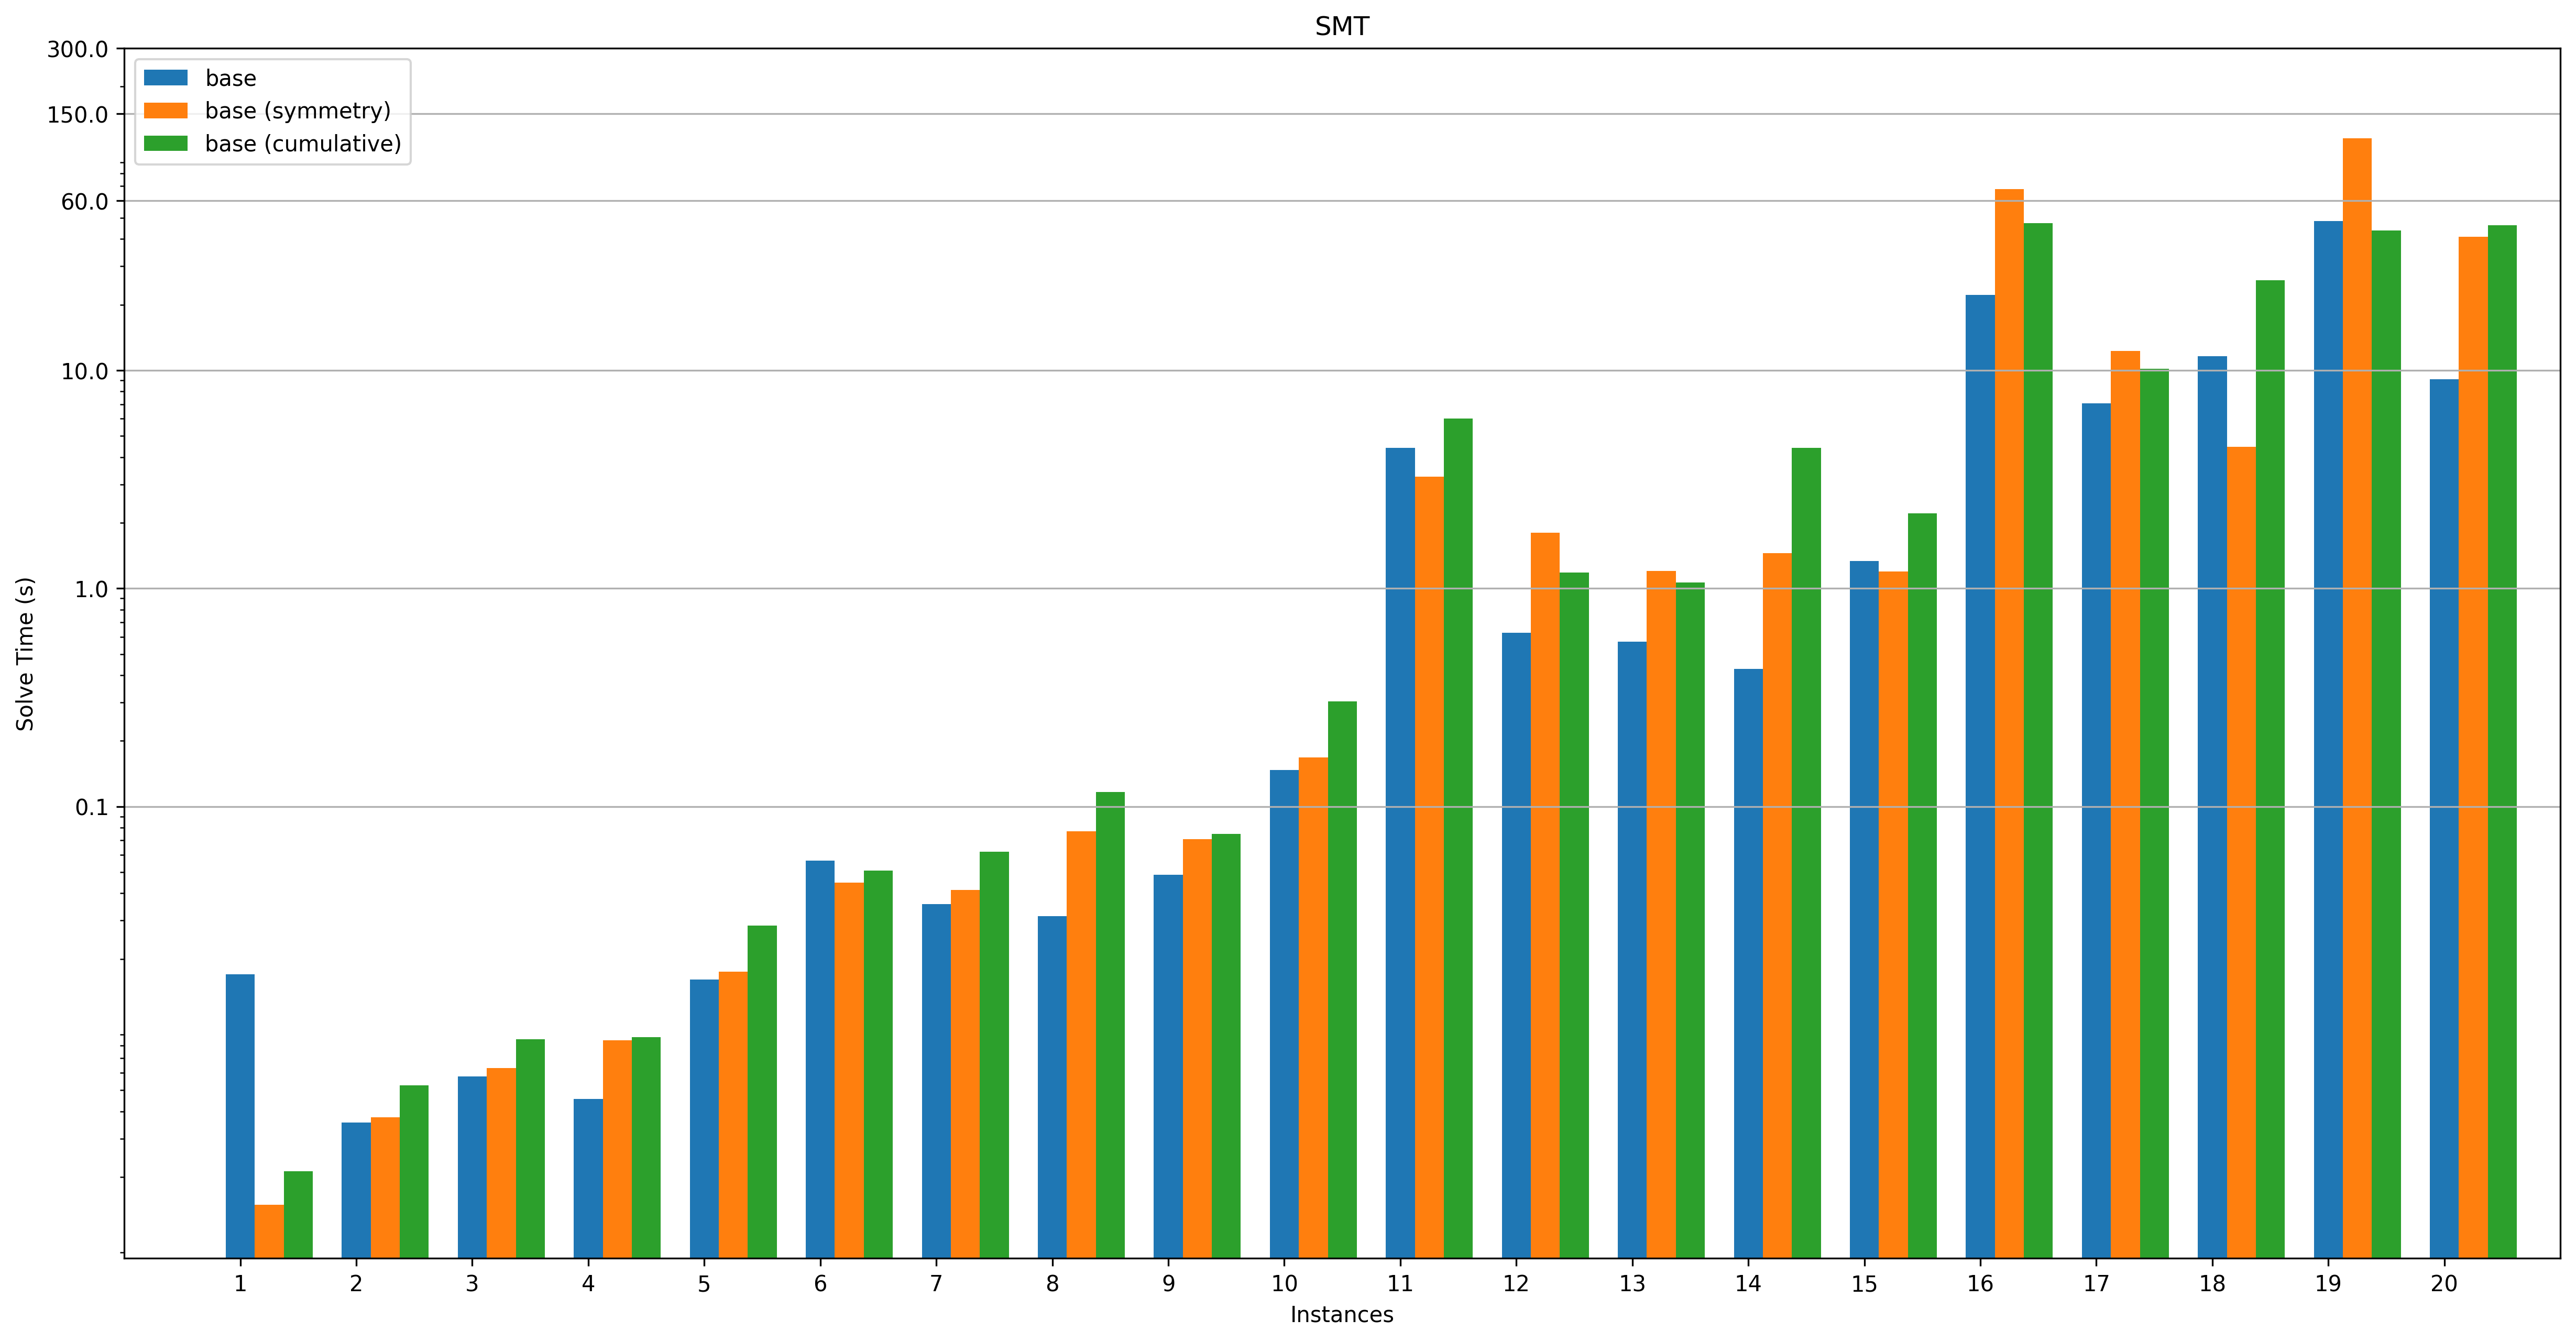
\includegraphics[width=\textwidth]{02/results_1.png}
    %         \caption{}
    %         \label{fig:vgpijerbgvpiberq}
    %     \end{subfigure}
    %     \begin{subfigure}[b]{1.0\textwidth}
    %         \centering
    %         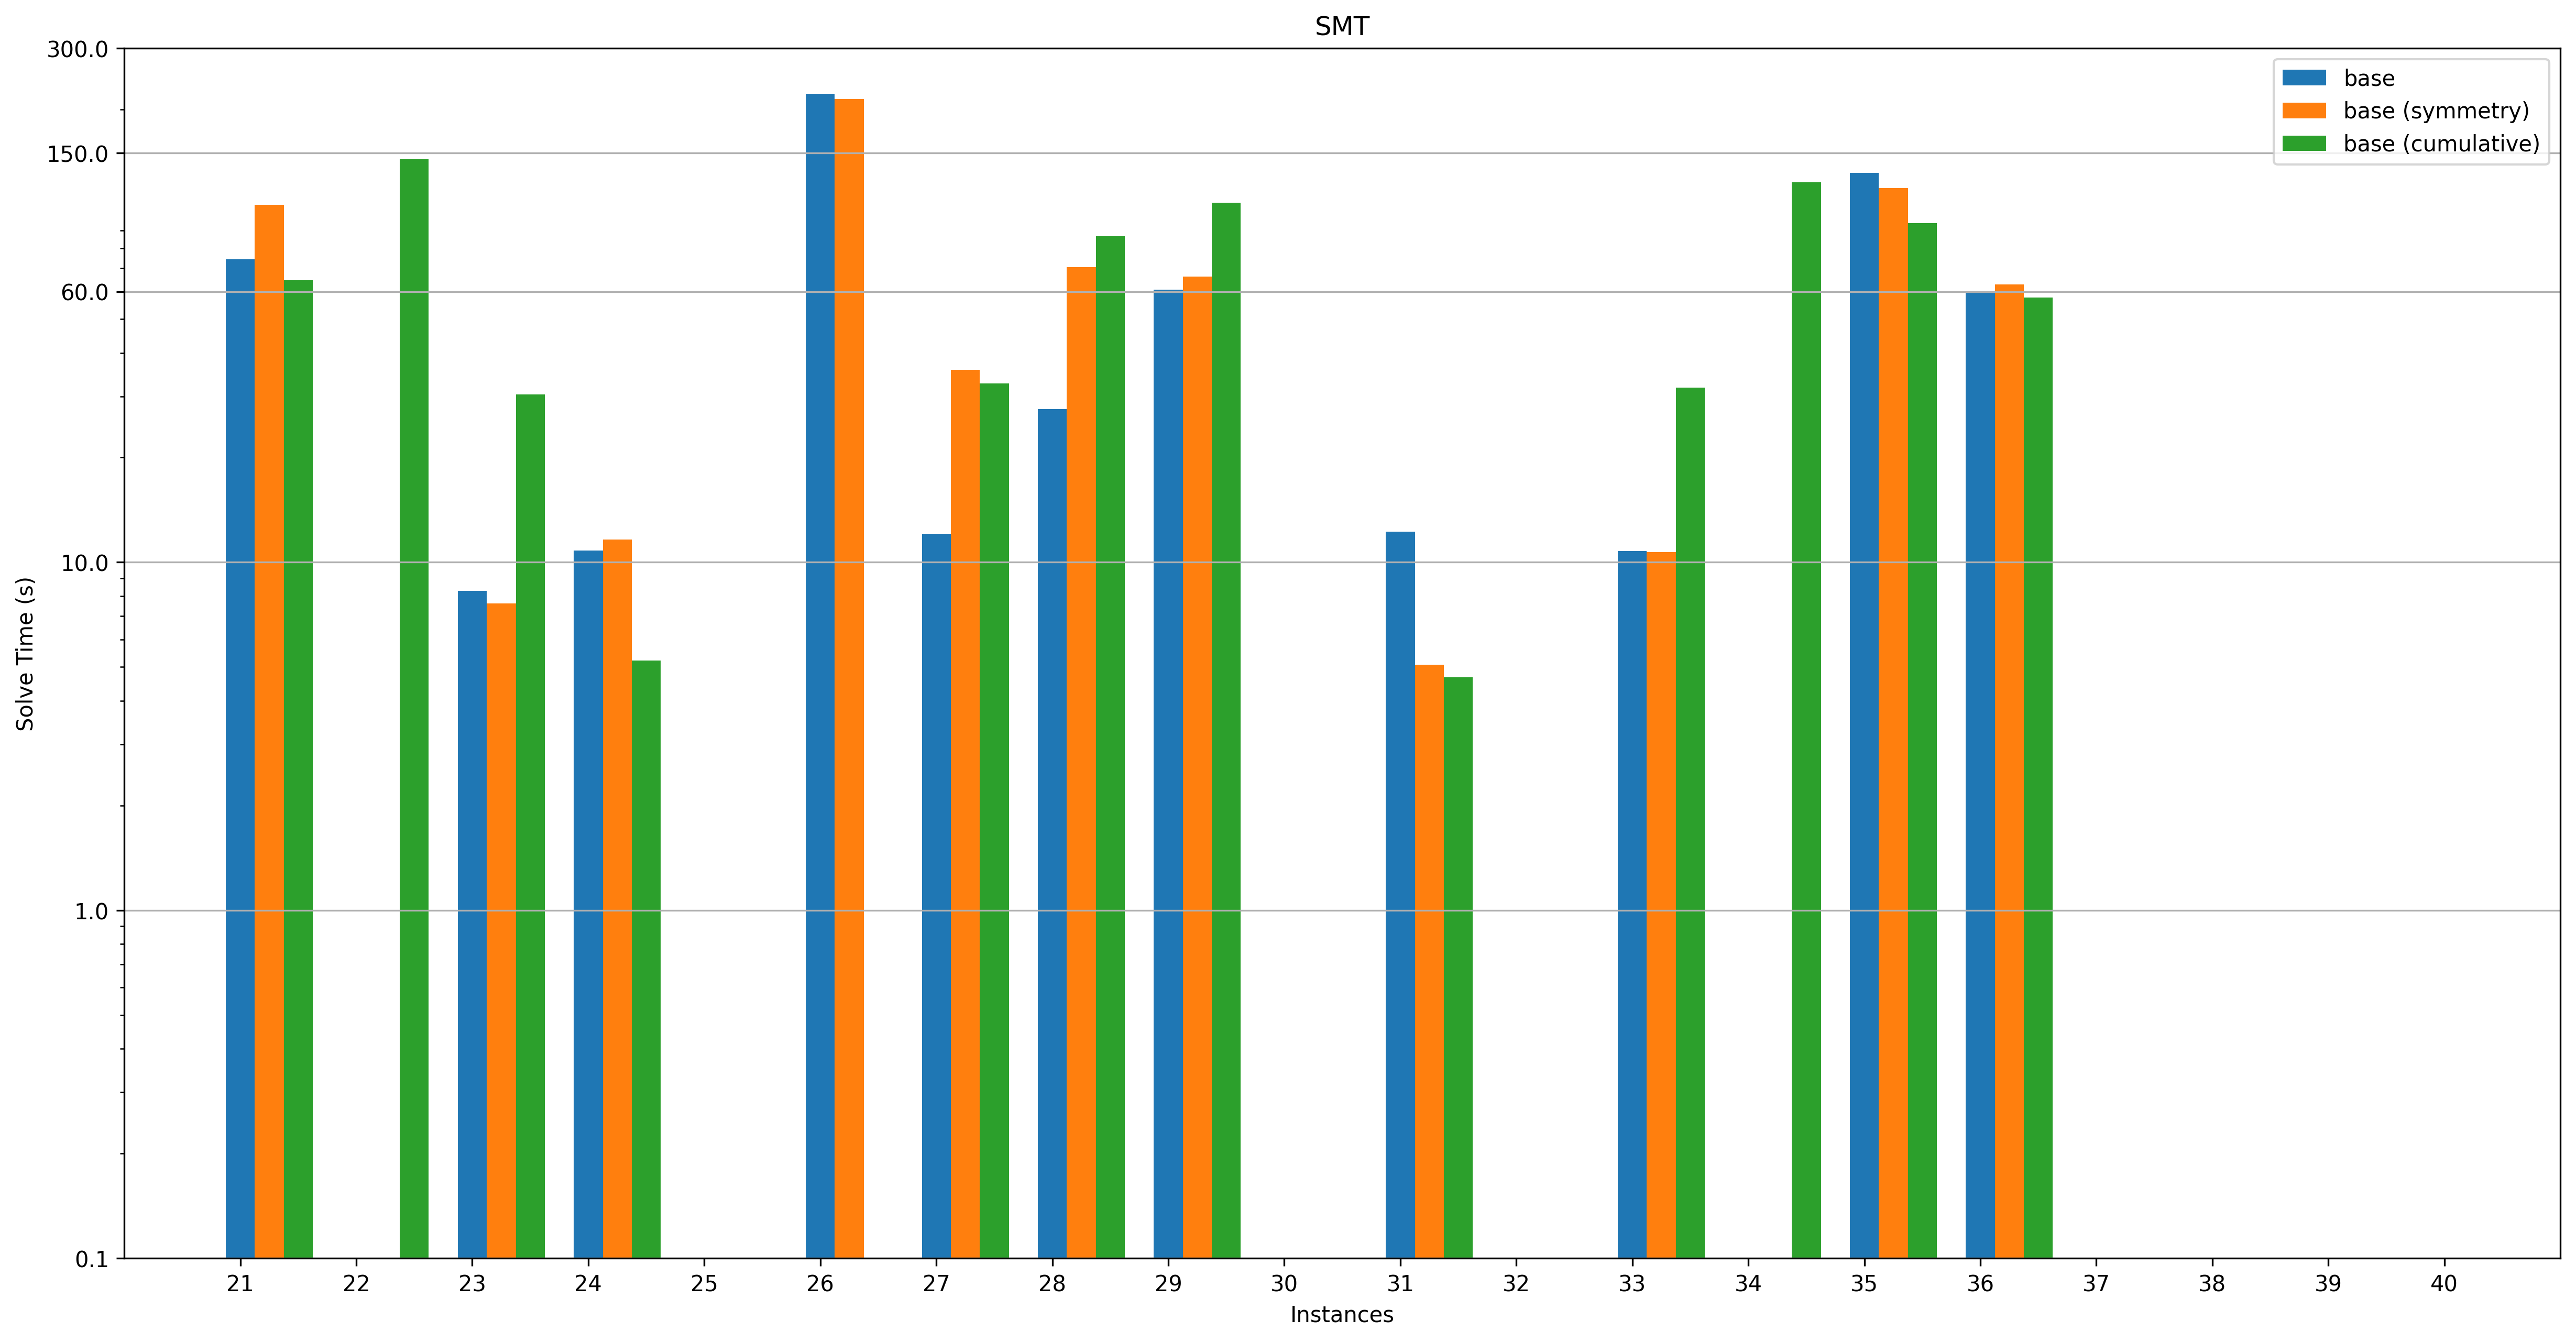
\includegraphics[width=\textwidth]{02/results_2.png}
    %         \caption{}
    %         \label{fig:vjidqenvjqen}
    %     \end{subfigure}
    %     \caption{weeeeeeeeeeee}
    %     \label{fig:vneqpwijvnpjewqnpivnenq}
    % \end{figure}

\subsection{Virtual Circuits}
    \colorbox{BurntOrange}{TODO missing ...}
